%___________________________
%===   Redéfinition des marges par défaut
%------------------------------------------------------
%\usepackage[textwidth=18.6cm]{geometry}%à mettre dans le preambule perso
%\pagestyle{fancy}%à mettre dans le preambule perso


\setlength\paperheight{297mm}
\setlength\paperwidth{210mm}
\setlength{\evensidemargin}{0cm}% Marge gauche sur pages paires
\setlength{\oddsidemargin}%{0cm}%
{-0.5cm}% Marge gauche sur pages impaires
\setlength{\topmargin}{-2cm}% Marge en haut
\setlength{\headsep}{0.5cm}% Entre le haut de page et le texte
\setlength{\headheight}{1cm}% Haut de page
\setlength{\textheight}{25.2cm}% Hauteur de la zone de texte
\setlength{\textwidth}{17cm}% Largeur de la zone de texte


% Environnement enumerate
\renewcommand{\theenumi}{\bf\textsf{\arabic{enumi}}}
\renewcommand{\labelenumi}{\bf\textsf{\theenumi.}}
\renewcommand{\theenumii}{\bf\textsf{\alph{enumii}}}
\renewcommand{\labelenumii}{\bf\textsf{\theenumii.}}
\renewcommand{\theenumiii}{\bf\textsf{\roman{enumiii}}}
\renewcommand{\labelenumiii}{\bf\textsf{\theenumiii.}}


\usetikzlibrary{shadows,trees}


%definition des couleurs
\definecolor{fondpaille}{cmyk}{0,0,0.1,0}%\pagecolor{fondpaille}
\definecolor{gris}{rgb}{0.7,0.7,0.7}
\definecolor{rouge}{rgb}{1,0,0}
\definecolor{bleu}{rgb}{0,0,1}
\definecolor{vert}{rgb}{0,1,0}
\definecolor{deficolor}{HTML}{2D9AFF}
\definecolor{backdeficolor}{HTML}{EDEDED}%{036DD0}%dégradé bleu{666666}%dégradé gris
\definecolor{theocolor}{HTML}{036DD0}%F4404D%rouge
\definecolor{backtheocolor}{HTML}{D3D3D3}
\definecolor{methcolor}{HTML}{008800}%12BB05}
\definecolor{backmethcolor}{HTML}{FFFACD}
\definecolor{backilluscolor}{HTML}{EDEDED}
\definecolor{sectioncolor}{HTML}{221E1E}%{B2B2B2}%vert : {HTML}{008800}%{HTML}{2D9AFF}
\definecolor{subsectioncolor}{HTML}{221E1E}%{B2B2B2}%vert : {HTML}{008800}%{rgb}{0.5,0,0}
\definecolor{engcolor}{HTML}{D4D7FE}
\definecolor{exocolor}{rgb}{0,0.6,0}
\definecolor{exosoltitlecolor}{rgb}{0,0.6,0}
\definecolor{titlecolor}{rgb}{1,1,1}

%commande pour enlever les couleurs avant impression
\newcommand{\nocolor}
{\pagecolor{white}
\definecolor{gris}{rgb}{0.7,0.7,0.7}
\definecolor{rouge}{rgb}{0,0,0}
\definecolor{bleu}{rgb}{0,0,0}
\definecolor{vert}{rgb}{0,0,0}
\definecolor{deficolor}{HTML}{B2B2B2}
\definecolor{backdeficolor}{HTML}{EEEEEE}%{036DD0}%dégradé bleu{666666}%dégradé gris
\definecolor{theocolor}{HTML}{B2B2B2}
\definecolor{backtheocolor}{HTML}{EEEEEE}
\definecolor{methcolor}{HTML}{B2B2B2}
\definecolor{backmethcolor}{HTML}{EEEEEE}
\definecolor{backilluscolor}{HTML}{EEEEEE}
\definecolor{sectioncolor}{HTML}{B2B2B2}
\definecolor{subsectioncolor}{HTML}{B2B2B2}
\definecolor{engcolor}{HTML}{EEEEEE}
\definecolor{exocolor}{HTML}{3B3838}
\definecolor{exosoltitlecolor}{rgb}{0,0,0}
\definecolor{titlecolor}{rgb}{0,0,0}
}



%___________________________
%===    Exercice résolu
%------------------------------------------------------
%
%#1 : énoncé
%#2 : solution
\newcounter{exosol}
\newcommand{\exosol}[2]{
\stepcounter{exosol}
\begin{tikzpicture}[node distance=0 cm]
\node[fill=backilluscolor,rounded corners=2pt,anchor=south west] (illus) at (0,-0.02)
{\it \textbf{\textcolor{exosoltitlecolor}{Exercice résolu \arabic{exosol}~:~}}};
\node[fill=backilluscolor,rounded corners=2pt,anchor=north west]at(0,0)
{\parbox{\columnwidth-10pt}{#1\par\medskip{\it \textbf{\textcolor{exosoltitlecolor}{Solution~:~}}}\par#2 }};
\end{tikzpicture}
\bigskip
}

\newcommand{\suite}[1]{
\begin{tikzpicture}[node distance=0 cm]
\node[fill=backilluscolor,rounded corners=2pt,anchor=north west]at(0,0)
{\parbox{\columnwidth-10pt}{{\it \textbf{\textcolor{exosoltitlecolor}{Suite de la solution~:}}}\par#1}};
\end{tikzpicture}
\bigskip
}



%%%%%%%%%%%%%%%%%%%%%%%%%%%%%%%%%%%%%%%%%%%%%%%%%%%%%%%%%%%%%%%%%%%%%%%%%%%%%%%
%Encadrés pour Propriétés, Théorème, Définitions, exemples, exercices

\usepackage{environ}%pour pouvoir utiliser la commande \NewEnviron

%___________________________
%===    Propriété avec ou sans s et avec ou sans titre
%------------------------------------------------------
%
\NewEnviron{Prop}[2][]{
\begin{tikzpicture}[node distance=0 cm]
\node[fill=theocolor,rounded corners=5pt,anchor=south west] (theorem) at (0,0)
{\textcolor{titlecolor}{Propriété#1~:~#2}};
\node[draw,drop shadow,color=theocolor,very thick,fill=backtheocolor,rounded corners=5pt,anchor=north west] at(0,-0.02)
{\black\parbox{\columnwidth-12pt}{\BODY}};
\end{tikzpicture}
\bigskip
}


%___________________________
%===    Conséquence avec ou sans s et avec ou sans titre
%------------------------------------------------------
%
\NewEnviron{Cons}[2][]{
\begin{tikzpicture}[node distance=0 cm]
\node[fill=theocolor,rounded corners=5pt,anchor=south west] (theorem) at (0,0)
{\textcolor{titlecolor}{Conséquence#1~:~#2}};
\node[draw,drop shadow,color=theocolor,very thick,fill=backtheocolor,rounded corners=5pt,anchor=north west] at(0,-0.02)
{\black\parbox{\columnwidth-12pt}{\BODY}};
\end{tikzpicture}
\bigskip
}


%___________________________
%===    Théorème avec ou sans titre
%------------------------------------------------------
%
\NewEnviron{Thm}[1][]{
\begin{tikzpicture}[node distance=0 cm]
\node[fill=theocolor,rounded corners=5pt,anchor=south west] (theorem) at (0,0)
{\textcolor{titlecolor}{Théorème~:~#1}};
\node[draw,drop shadow,color=theocolor,very thick,fill=backtheocolor,rounded corners=5pt,anchor=north west] at(0,-0.02)
{\black\parbox{\columnwidth-12pt}{\BODY}};
\end{tikzpicture}
\medskip
}


%___________________________
%===    Cadre arrondi coloré
%------------------------------------------------------
%
\NewEnviron{CadreColor}{

\begin{tikzpicture}[node distance=0 cm]
\node[draw,drop shadow,color=theocolor,very thick,fill=backtheocolor,rounded corners=5pt,anchor=north west] at(0,-0.02)
{\black\parbox{\columnwidth-12pt}{\BODY}};
\end{tikzpicture}
\medskip
}


%___________________________
%===    Cadre arrondi blanc
%------------------------------------------------------
%
\NewEnviron{Cadre}{
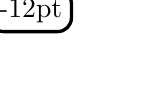
\begin{tikzpicture}[node distance=0 cm]
\node[draw,very thick,rounded corners=5pt,anchor=north west] at(0,-0.02)
{\black\parbox{\columnwidth-12pt}{\BODY}};
\end{tikzpicture}
\medskip
}



%___________________________
%===    Règle(s) avec ou sans s et avec sans titre
%------------------------------------------------------
%
\NewEnviron{Regle}[2][]{
\begin{tikzpicture}[node distance=0 cm]
\node[fill=theocolor,rounded corners=5pt,anchor=south west] (theorem) at (0,0)
{\textcolor{titlecolor}{Règle#1~:~#2}};
\node[draw,drop shadow,color=deficolor,very thick,fill=backdeficolor,rounded corners=5pt,anchor=north west] at(0,-0.02)
{\black\parbox{\columnwidth-12pt}{\BODY}};
\end{tikzpicture}
\medskip
}

%___________________________
%===    Définition avec ou sans s et avec sans titre
%------------------------------------------------------
%
\NewEnviron{Defi}[2][]{
\begin{tikzpicture}[node distance=0 cm]
\node[fill=theocolor,rounded corners=5pt,anchor=south west] (theorem) at (0,0)
{\textcolor{titlecolor}{Définition#1~:~#2}};
\node[draw,drop shadow,color=deficolor,very thick,fill=backdeficolor,rounded corners=5pt,anchor=north west] at(0,-0.02)
{\black\parbox{\columnwidth-12pt}{\BODY}};
\end{tikzpicture}
\medskip
}

%___________________________
%===    Méthode avec ou sans s et avec sans titre
%------------------------------------------------------
%
\NewEnviron{Methode}[2][]{
\begin{tikzpicture}[node distance=0 cm]
\node[fill=theocolor,rounded corners=5pt,anchor=south west] (theorem) at (0,0)
{\textcolor{titlecolor}{Méthode#1~:~#2}};
\node[draw,drop shadow,color=methcolor,very thick,fill=backmethcolor,rounded corners=5pt,anchor=north west] at(0,-0.02)
{\black\parbox{\columnwidth-12pt}{\BODY}};
\end{tikzpicture}
\medskip
}


%___________________________
%===    Redéfinition de la commande \chapter{•}
%------------------------------------------------------
%
\makeatletter

\renewcommand{\@makechapterhead}[1]{
\begin{tikzpicture}
\node[fill=theocolor,rectangle,rounded corners=5pt]{%
\begin{minipage}{\linewidth}
\begin{center}
\vspace*{9pt}
\textcolor{titlecolor}{\Large \textsc{\textbf{Chapitre \thechapter \ : \ #1}}}
\vspace*{9pt}
\end{center}
\end{minipage}
};\end{tikzpicture}
}

\makeatother


%___________________________
%===    Exemple avec ou sans s et avec ou sans titre
%------------------------------------------------------
%
\NewEnviron{Exemple}[2][]{
\begin{tikzpicture}[node distance=0 cm]
\node[draw,drop shadow,color=methcolor,very thick,fill=backmethcolor,rounded corners=5pt,anchor=north west] at(0,-0.02)
{\black\parbox{\columnwidth-12pt}{\textbf{Exemple#1~:~#2}\\
\BODY}};
\end{tikzpicture}
\medskip
}

%___________________________
%===    Remarque avec ou sans s
%------------------------------------------------------
%
\NewEnviron{Rmq}[1][]{
\textbf{\large{Remarque#1 :}}\par
\BODY
\medskip
}

%___________________________
%===    Remarques numérotées R1, R2, etc...
%------------------------------------------------------
%
\newcounter{rem}\newcommand{\rem}{\refstepcounter{rem}\textbf{R \therem \ :}\xspace}

%___________________________
%===    Exercices du contrôle numérotés
%------------------------------------------------------
%
\newcounter{exercice}
\NewEnviron{Exercice}[1][]{
\refstepcounter{exercice}\textbf{\large{Exercice \theexercice \ :}}\hfill \textbf{#1}\par
\BODY
\medskip
}

%___________________________
%===    Exercices non numérotés
%------------------------------------------------------
%
\NewEnviron{Exo}[1][]{
\textbf{\large{Exercice #1 \ :}}\par
\BODY
\medskip
}

%___________________________
%===    Démonstration
%------------------------------------------------------
\NewEnviron{Demo}{%
\textit{\textbf{Démonstration.}}\par
\BODY
\strut\hfill$\square$
\medskip
}

%___________________________
%===    Commandes perso
%------------------------------------------------------
%
%\Leftrightarrow
\newcommand{\Lr}{\Leftrightarrow}

%Ancienne commande chapitre
\newcommand{\chapitre}[1]{
\begin{tikzpicture}
\node[fill=theocolor,rectangle,rounded corners=5pt]{%
\begin{minipage}{\linewidth}
\begin{center}
\vspace*{9pt}
\textcolor{titlecolor}{\Large \textsc{\textbf{#1}}}
\vspace*{9pt}
\end{center}
\end{minipage}
};
\end{tikzpicture}
\bigskip
}

%Pour les fiches : commande de Cécile
\newcommand{\Fiche}[2]{%
\begin{tikzpicture}
	\node[draw, color=blue,fill=white,rectangle,rounded corners=5pt]{%
	\begin{minipage}{\linewidth}
		\begin{center}
			\vspace*{9pt}
			\textcolor{blue}{\Large \textsc{\textbf{Fiche~#1\ :\ #2}}}
			\vspace*{7pt}
		\end{center}
	\end{minipage}
	};
\end{tikzpicture}
}%

\pagecolor{white}%couleur du fond de page

\renewcommand{\Pointilles}{%
\makebox[\linewidth]{\dotfill}
}


%centrer du texte ou une formule avec moins d'espace autour
\newcommand{\centrer}[1]
{
\smallskip
\centerline{#1}
\smallskip
}


%QRcode généré par le package qrcode
\usepackage{qrcode}


%Pour pouvoir utiliser l'environnement verbatim
\usepackage{verbatim}

%Panneau danger (nécessite le package pstricks)
\def\danger{\begingroup
\psset{unit=1ex}%
\begin{pspicture}(0,0)(3,3)
 
\pspolygon[linearc=0.2,linewidth=0.12,linecolor=red](0,0)(1.5,2.6)(3,0)
 
\psellipse*(1.5,1.33)(0.14,0.75)\pscircle*(1.5,0.3){0.15}\end{pspicture}
%
\endgroup}%

%___________________________
%===    Nouvelles commandes pour documents venant de Sesamath
%------------------------------------------------------
%
\definecolor{CyanTikz40}{cmyk}{.4,0,0,0}
\definecolor{CyanTikz20}{cmyk}{.2,0,0,0}
\tikzstyle{general}=[line width=0.3mm, >=stealth, x=1cm, y=1cm,line cap=round, line join=round]
\tikzstyle{quadrillage}=[line width=0.3mm, color=CyanTikz40]
\tikzstyle{quadrillageNIV2}=[line width=0.3mm, color=CyanTikz20]
\tikzstyle{quadrillage55}=[line width=0.3mm, color=CyanTikz40, xstep=0.5, ystep=0.5]
\tikzstyle{cote}=[line width=0.3mm, <->]
\tikzstyle{epais}=[line width=0.5mm, line cap=butt]
\tikzstyle{tres epais}=[line width=0.8mm, line cap=butt]
\tikzstyle{axe}=[line width=0.3mm, ->, color=Noir, line cap=rect]
\newcommand{\quadrillageSeyes}[2]{\draw[line width=0.3mm, color=A1!10, ystep=0.2, xstep=0.8] #1 grid #2;
\draw[line width=0.3mm, color=A1!30, xstep=0.8, ystep=0.8] #1 grid #2; }
\newcommand{\axeX}[4][0]{\draw[axe] (#2,#1)--(#3,#1); \foreach \x in {#4} {\draw (\x,#1) node {\small $+$}; \draw (\x,#1) node[below] {\small $\x$};}}
\newcommand{\axeY}[4][0]{\draw[axe] (#1,#2)--(#1,#3); \foreach \y in {#4} {\draw (#1, \y) node {\small $+$}; \draw (#1, \y) node[left] {\small $\y$};}}
\newcommand{\axeOI}[3][0]{\draw[axe] (#2,#1)--(#3,#1);  \draw (1,#1) node {\small $+$}; \draw (1,#1) node[below] {\small $I$};}
\newcommand{\axeOJ}[3][0]{\draw[axe] (#1,#2)--(#1,#3); \draw (#1, 1) node {\small $+$}; \draw (#1, 1) node[left] {\small $J$};}
\newcommand{\axeXgraduation}[2][0]{\foreach \x in {#2} {\draw (\x,#1) node {\small $+$};}}
\newcommand{\axeYgraduation}[2][0]{\foreach \y in {#2} {\draw (#1, \y) node {\small $+$}; }}
\newcommand{\origine}{\draw (0,0) node[below left] {\small $0$};}
\newcommand{\origineO}{\draw (0,0) node[below left] {$O$};}
\newcommand{\point}[4]{\draw (#1,#2) node[#4] {$#3$};}
\newcommand{\pointGraphique}[4]{\draw (#1,#2) node[#4] {$#3$};
\draw (#1,#2) node {$+$};}
\newcommand{\pointFigure}[4]{\draw (#1,#2) node[#4] {$#3$};
\draw (#1,#2) node {$\times$};}
\newcommand{\pointC}[3]{\draw (#1) node[#3] {$#2$};}
\newcommand{\pointCGraphique}[3]{\draw (#1) node[#3] {$#2$};
\draw (#1) node {$+$};}
\newcommand{\pointCFigure}[3]{\draw (#1) node[#3] {$#2$};
\draw (#1) node {$\times$};}


\definecolor{B1prime}                {cmyk}{0.00, 1.00, 0.00, 0.50}
\definecolor{H1prime}                {cmyk}{0.50, 0.00, 1.00, 0.00}

\definecolor{FootFonctionColor}{cmyk}{0.50, 0.00, 0.00, 0.00}
\definecolor{FootGeometrieColor}{cmyk}{0.40, 0.40, 0.00, 0.00}
\definecolor{FootStatistiqueColor}{cmyk}{0.30, 0.48, 0.00, 0.10}
\definecolor{FootStatistiqueOLDColor}{cmyk}{0.48, 0.30, 0.10, 0.00}
\definecolor{FootStatistique*Color}{cmyk}{0.20, 0.00, 0.00, 0.00}
\definecolor{ActiviteFootColor}{cmyk}{0.50, 0.00, 0.25, 0.00}
\definecolor{CoursFootColor}{cmyk}{0.15, 0.00, 0.00, 0.03}
\definecolor{ExoBaseFootColor}{cmyk}{0.00, 0.25, 0.50, 0.00}
\definecolor{ExoApprFootColor}{cmyk}{0.00, 0.25, 0.50, 0.00}
%\colorlet{ConnFootColor}{F2}
\definecolor{TPFootColor}{cmyk}{0.00, 0.30, 0.00, 0.10}
\definecolor{RecreationFootColor}{cmyk}{0.20, 0.00, 0.50, 0.05}

\definecolor{Blanc}             {cmyk}{0.00, 0.00, 0.00, 0.00}
\definecolor{Gris1}             {cmyk}{0.00, 0.00, 0.00, 0.20}
\definecolor{Gris2}             {cmyk}{0.00, 0.00, 0.00, 0.40}
\definecolor{Gris3}             {cmyk}{0.00, 0.00, 0.00, 0.50}
\definecolor{Noir}              {cmyk}{0.00, 0.00, 0.00, 1.00}
\definecolor{A1}              {cmyk}{0.33, 1.00, 0.00, 0.40}
\definecolor{F1}              {cmyk}{0.00, 1.00, 1.00, 0.00}
\definecolor{C1}              {cmyk}{0.00, 1.00, 0.00, 0.50}
\definecolor{G1}              {cmyk}{0.00, 0.00, 0.00, 0.20}
\definecolor{D1}              {cmyk}{0.00, 0.22, 0.49, 0.69}%bitume
\definecolor{J1}              {cmyk}{0.00, 0.34, 1.00, 0.02}%orangé


%augmenter l'espace au-dessus ou en-dessous d'une fraction
\usepackage{fixltx2e}
\makeatletter
\newcommand*\Strut[1][1]{%
  \leavevmode
  \vrule \@height #1\ht\strutbox
         \@depth #1\dp\strutbox
         \@width\z@
}
\newcommand*\TopStrut[1][1]{%
  \leavevmode
  \vrule \@height #1\ht\strutbox
         \@depth \z@
         \@width \z@
}
\newcommand*\BotStrut[1][1]{%
  \leavevmode
  \vrule \@height \z@
         \@depth #1\dp\strutbox
         \@width \z@
}
\makeatother
%%%%%%%%%%%%%%%%%%%%%%%%%%%%%%%%%%%%%%%%%%%%%%%%%%%%%%%%%%%%%%%%%%%%%%%%%%%%%%%